% Explain the implementaiton of the debug adapeter

% Overview description of the debug adapter and the flow of communication from the user to the debugger.
The debug adapter is implemented as a \gls{tcp} server in the main thread.
It starts a debug thread when a new \gls{tcp} connection is made.
After that it starts listening for \gls{dap} messages on the \gls{tcp} connection.


The first \gls{dap} messages are for communicating the \gls{dap} functionalities that the client and the debugger has.
These first \gls{dap} messages also contain some configuration for the debug thread, those configuration are forwarded to the debug thread.
After that the debug adapter will continuously pull for messages from the \gls{tcp} client and the debug thread, until a message is received.


When the debug adapter receives a \gls{dap} message from the server it translates it to one or more commands for the debug thread.
Those commands are then sent one by one to the debug thread.
The responses from those commands are then used to make the response to the client.
If the main thread gets a event from the debug thread it will translate it into a \gls{dap} message and send it to the client.



%% Add a flow cart of the communication? % TODO
%\begin{figure}[h]
%	\centering
%	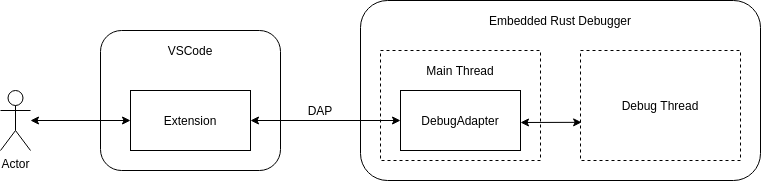
\includegraphics[width=0.9\textwidth]{user_dap_debug.png}
%	\caption{A diagram showing the comunication between the user/actor, \emph{VSCode} and the debugger \emph{Embedded Rust Debugger}.}
%	\label{fig:userDAP}
%\end{figure}


%\subsubsubsection{Initial \acrshort{dap} Messages}
%% Initializing the connection % TODO
%It is required the the first few \acrshort{dap} messages sent to the debug adapter is for configuring the debug adapter by communicating the supported capabilities of the debugger and \emph{VSCode}.
%This debugger doesn't support any of the optional capabilities that are defined in the \acrshort{dap} protocol and will thus not show up in \emph{VSCode}.
%After everything is configured then the debugger will get a requires to flash the connected debug target with the program that is going to be debugged.
%Now the debug adapter is started and will work as a middle man between the debugger and the \acrshort{gui}.
%
%
%\subsubsubsection{Translating \acrshort{dap} Messages To Internal Messages}
%% Explain how the debug adapter converts the DAP messages to instructions for the debugger. % TODO: remove this paragraph?
%The debug adapter and the debugger is running on separate threads and thus communicate asynchronously using channels.
%The channels uses a different set of commands then that is defined in \acrshort{dap} which means that the debug adapter translates these commands and forwards them.
%This means that a single \acrshort{dap} message can result in multiple commands being sent from the debug adapter to the debugger.
%
%
%\subsubsubsection{Simultaneous Handling Of \acrshort{dap} Messages And Events}
%% Explaining how the debug adapter communicate with the debugger and wise versa. % TODO
%Because the debug adapter can get messages from both the \acrshort{gui} and the debugger at any time it uses continues polling on the \gls{tcp} connection and the channel.
%This enables the debug adapter to forward messages sent by both \emph{VSCode} and the debugger.

